\documentclass[12pt onesided letterpaper]{article}
\usepackage{graphicx}
\usepackage{hyperref}
\title{Headmaster: A Dream Interface}
\author{Kaitlyn Higa\\
        CMSI370}
\date{November 29, 2012}
\begin{document}
\maketitle
\section*{Introduction}
Headmaster is an application that just screams to be implemented on a mobile, touch-based platform.  The system itself is designed to keep records of all of the student body, which itself is not stationary or based solely around a classroom.  With all of its administrative information, such as Student's information, Events, and Grants, Headmaster would prove to be a viable resource to be available at one's fingertips at a seconds notice. Mobility is key in today's world; as technology moves forward, the push for easy-access, portable devices is strengthened.  No one has time to be tethered down to a power cord, or even to sit down with a laptop.  Physical keyboards have been replaced with on-screen ones; mice have been nixed in favor of the touchscreen. Thus, the next step for the Headmaster system is to be designed for a mobile, touch-based platform.   
\\
All administrative offices will be equipped with a set of 20 iPads, which are each outfitted with a fingerprint scanner.  Each of these will be loaded with and are completely dedicated to the Headmaster system.  In order to check out an iPad, one must scan their fingerprint.  This will give the appropriate permissions to that user.  Additionally, the system can be used on personal touch-based devices that are registered on the network to their individual users. The device will simply use a MYLMU login to confirm the identity of the user.

\section*{The Headmaster System}
The Headmaster System is a system in which a user can access student information including all academic records as well as information about grants and events.  There will be three types of accounts, professor/instructor, administrators, students.  All three can change student information, but the student and their student advisor must approve.  Deans of colleges can override all three.  Changes made in the Headmaster system will directly change Student records.


\section*{Home Screen}
The home screen includes a toolbar, and a fixed, non-scrolling menu that links to the features of the Headmaster system, that is, the students, events, grants, and extended class list.  
\\
Whenever the user interacts with the system, he or she will constantly be receiving feedback.  By tapping an item, the system should respond with haptic feedback, default audio for a tap, and the button in question should change color. A swipe will respond with haptic feedback on finger-down, the default audio for a swipe, and an animation, showing the object being swiped. For consistency (Smith and Mosier 1986)\cite{dondi12} all of these should remain the same throughout the system.
\\
\subsection*{Toolbar}
In order to create consistency (Smith and Mosier 1986)\cite{dondi12} a toolbar is fixed to the top of each page. The toolbar at the top will always contain the date, time, a link to the home page, a log out button, and a search function, mostly all represented with symbols.  There will also be a pull-down menu in which everything can be accessed through in textual form, accessed by pulling down on the toolbar wherever there is no text or symbols.  This is with the World Wide Web Consortium's guideline that states “Provide a text equivalent for every non-text element.” The home page button will be represented by a house symbol and the log out button will be represented by a power symbol.  The home page symbol will appear next to the search bar symbol on the right-most side of the toolbar whereas the log out symbol will be on the left most side, to lessen errors(i.e. accidental log out).     
\\
\subsection*{Search Bar}
The search bar will be compacted to a magnifying glass symbol until use to save space within the toolbar.  The search bar will feature voice input, as well as predictions, so that the user can create input in a variety of different methods.  In this manner, the user can utilize vocal commands, command line controls, and will have a sense of recollection with the prediction/suggestion bar. The predictions/suggestions will list all list organizers, such as College, Year, or Clubs. 
\\
\subsection*{Students Menu}
The Students menu on the homepage will be a box that spans the width of the screen and takes up about a third of the page.  Within it, it will contain a search icon (which expands to a bar when clicked) which is specifies its search to the student base only (meaning that it excludes grants, classes, and events) as well as dropdown menus that will organize students by College or Year. 
\\
\subsection*{Events Menu}
The Events menu on the homepage will be a box that spans the width of the screen and takes up the second third of the stage.  It too will contain a search search icon  that is limited to the events searchable base. Below that, the three next upcoming events will appear.  On the bottom most right corner of the box, a dropdown with the previous/next 6 months will appear.  If tapped in the header, the Events page will appear; if on the search symbol, the cursor in the search bar will appear and the keyboard will come up, and if an event is tapped on, details for that event will appear. If a month in the dropdown is selected, the Event page with the events from that calendar month will appear.
\\
\subsection*{Classes Menu}
The Classes menu on the homepage will be a box that spans half the width of the screen and is in the last third of the page.  Again, it will have a search symbol which reveals a search bar when tapped. The box will have options to search via Map, which will show which classes are being held where, as well as a bulletin search, which organizes the classes into a heirarchy.
\\
\subsection*{Grants Menu}
The Grants menu on the homepage will be a box that spans half the width of the screen and is in the last third of the page, opposite the Classes menu.  It will have a search symbol which reveals a search bar when tapped. The box will have options to search via Map, which will show which classes are being held where, as well as a bulletin search, which organizes the classes into a heirarchy.
\\
\subsection*{Organization}
The home screen can be customized in a direct manipulation manner.  An option to reorganize will appear on the pull-down menu, and a small move cursor symbol will be in the lower right corner.  The designs are limited to two large bars with two smaller half screen bars.  All can be half screened for a total of two bars.  The settings are saved to the individual user account.  
\\
\subsection*{Design}
The home screen also incorporates a simple swiss style design, with a bootstrap-y asthetic.  Since Headmaster is mainly meant to send/retrieve information about students, I feel a simpler design would not only run more efficiently but also create an experience that is well liked because it is so straightforward. This choice, I believe will reduce short-term memory load, a principle touted by both Schniderman and Nielson. In addition, it will be easier to create because of the fact that swiss style design is based off the idea of utilizing grids in creating typographical-centric design.\cite{terror09} 

\\
\section*{Search Screen}
The search screen will appear once a user has searched for something via a search bar.  It will display in a list format, grouping together things classified as either Students, Classes, Grants, or Events.  An advanced search can be done as well, with restrictions that refine searches or certain categories or even subcategories, like searching by college or major.  

\section*{Student Screen}
The student page details all specifics about the student, including all of the features already implemented in the current Headmaster system.  All of what is currently being implemented within the Headmaster web-app will be included here.   The toolbar appears at the top, like every other page.  All of the student's basic information, his or her name, year, college, major, and with a head shot, is fixed in a container that is the first top quarter of the page.  There will be a big button to edit on the right most side of the container, away from every other element in the box.  The edit option will also be available in the pull-down menu.  There will also be a sidebar that takes up a quarter of the page with direct links to the information contained within the page, like GPA, schedule, grants, extra curriculars, food allergies, etc. Instead of the two columns featured in the web-app, the information will be implemented in a single, scrollable container which takes up the rest of the page.  
The Students can be looked at, grouped by year or college.  If the user decides to group by year, Freshmen will appear first, in alphabetical order.  If the user decides to group by college, the students will be organized by major alphabetically.  A head shot along with a the student's name, major, and year will be used to represent them. To select a student, the user can tap the photo or swipe the container that has the user's information to the right. 

\section*{Event Screen}
The event page will default to a screen split with a top container(top quarter) that has events that a user can swipe through and a bottom container(bottom three-quarters) that has a calendar view with all the events listed, that the user has permissions to view.  A large plus sign next to the “Events” title can be used for creating new events.  An option to add an event would also be added to the pull-down menu.  The top container would feature the next upcoming events, and the user would flick either left or right to see the next(swipe left) or previous(swipe right) event.  The calendar will also be able to flip back and forth, but the user will swipe up to reveal the next month, and swipe down to reveal the previous month. There will be options to connect these events with Google and/or Facebook calendar.


\section*{Grants Screen}
The grants screen contains an accordion-like, hierarchical menu which provides several classifications for types of grants.  From here, you can select a grant, and a description about the grant will appear.  A student can apply for the grant or you can choose to see who already has the grant, which will return a selected students page, with those who are receiving said grant visible. 

\section*{Classes Screen}
The classes screen has two possible settings.  A toggle switch just below the toolbar will dictate which of the two states the classes screen is in.  An option on the pull-down menu, with a pop-up containing  radio buttons will be added.  

\subsection*{The Bulletin Setting}
The first setting is the bulletin setting, in which all classes can be viewed.  A dropdown at the top of the page details hierarchical organizations, like by college and major or by program and professors. You can expand or collapse sections and are able to access the bulletin similar to the one already implemented at \url{'http://bulletin.lmu.edu/'}
\\
\subsection*{The Map Setting}
The second setting is the Map setting.  A map of LMU campus will appear on the screen, and you can click on a building to see what classes are happening at that time.  By default, the map will give you the course being held in a classroom at that time and date, but via a limited input box, you can change what times/days you're looking at.  Another toggle setting near the top will turn on the physical classroom setting.
\\
\subsection*{The Physical Classroom Setting}
When a person enters a classroom, the iPad will automatically sense the location via a short-range Bluetooth transmitter which will broadcast the location of the room.  Based upon the time and classroom location, Headmaster will retrieve a roster for the appropriate users, namely the instructor of the course or an administrator.  For an instructor, the roster appears along with the MYLMUConnect course page.  From the roster, the instructor is able to access student pages by simply swiping the student's information or taping their photo.  If Headmaster is logged on with a student account, it will provide only course information which would detail prerequisites, instructors, times, and avaliability. If that student is enrolled in the course, the MYLMUConnect course page will appear. It will also register that the student is present on the instructor's roster. Alternatively, if that student is supposed to be in a different class, a warning will appear telling the student that he or she is in the incorrect classroom.  
\\
\begin{figure}[h!]
  \caption{An Instructor's view.}
  \centering
    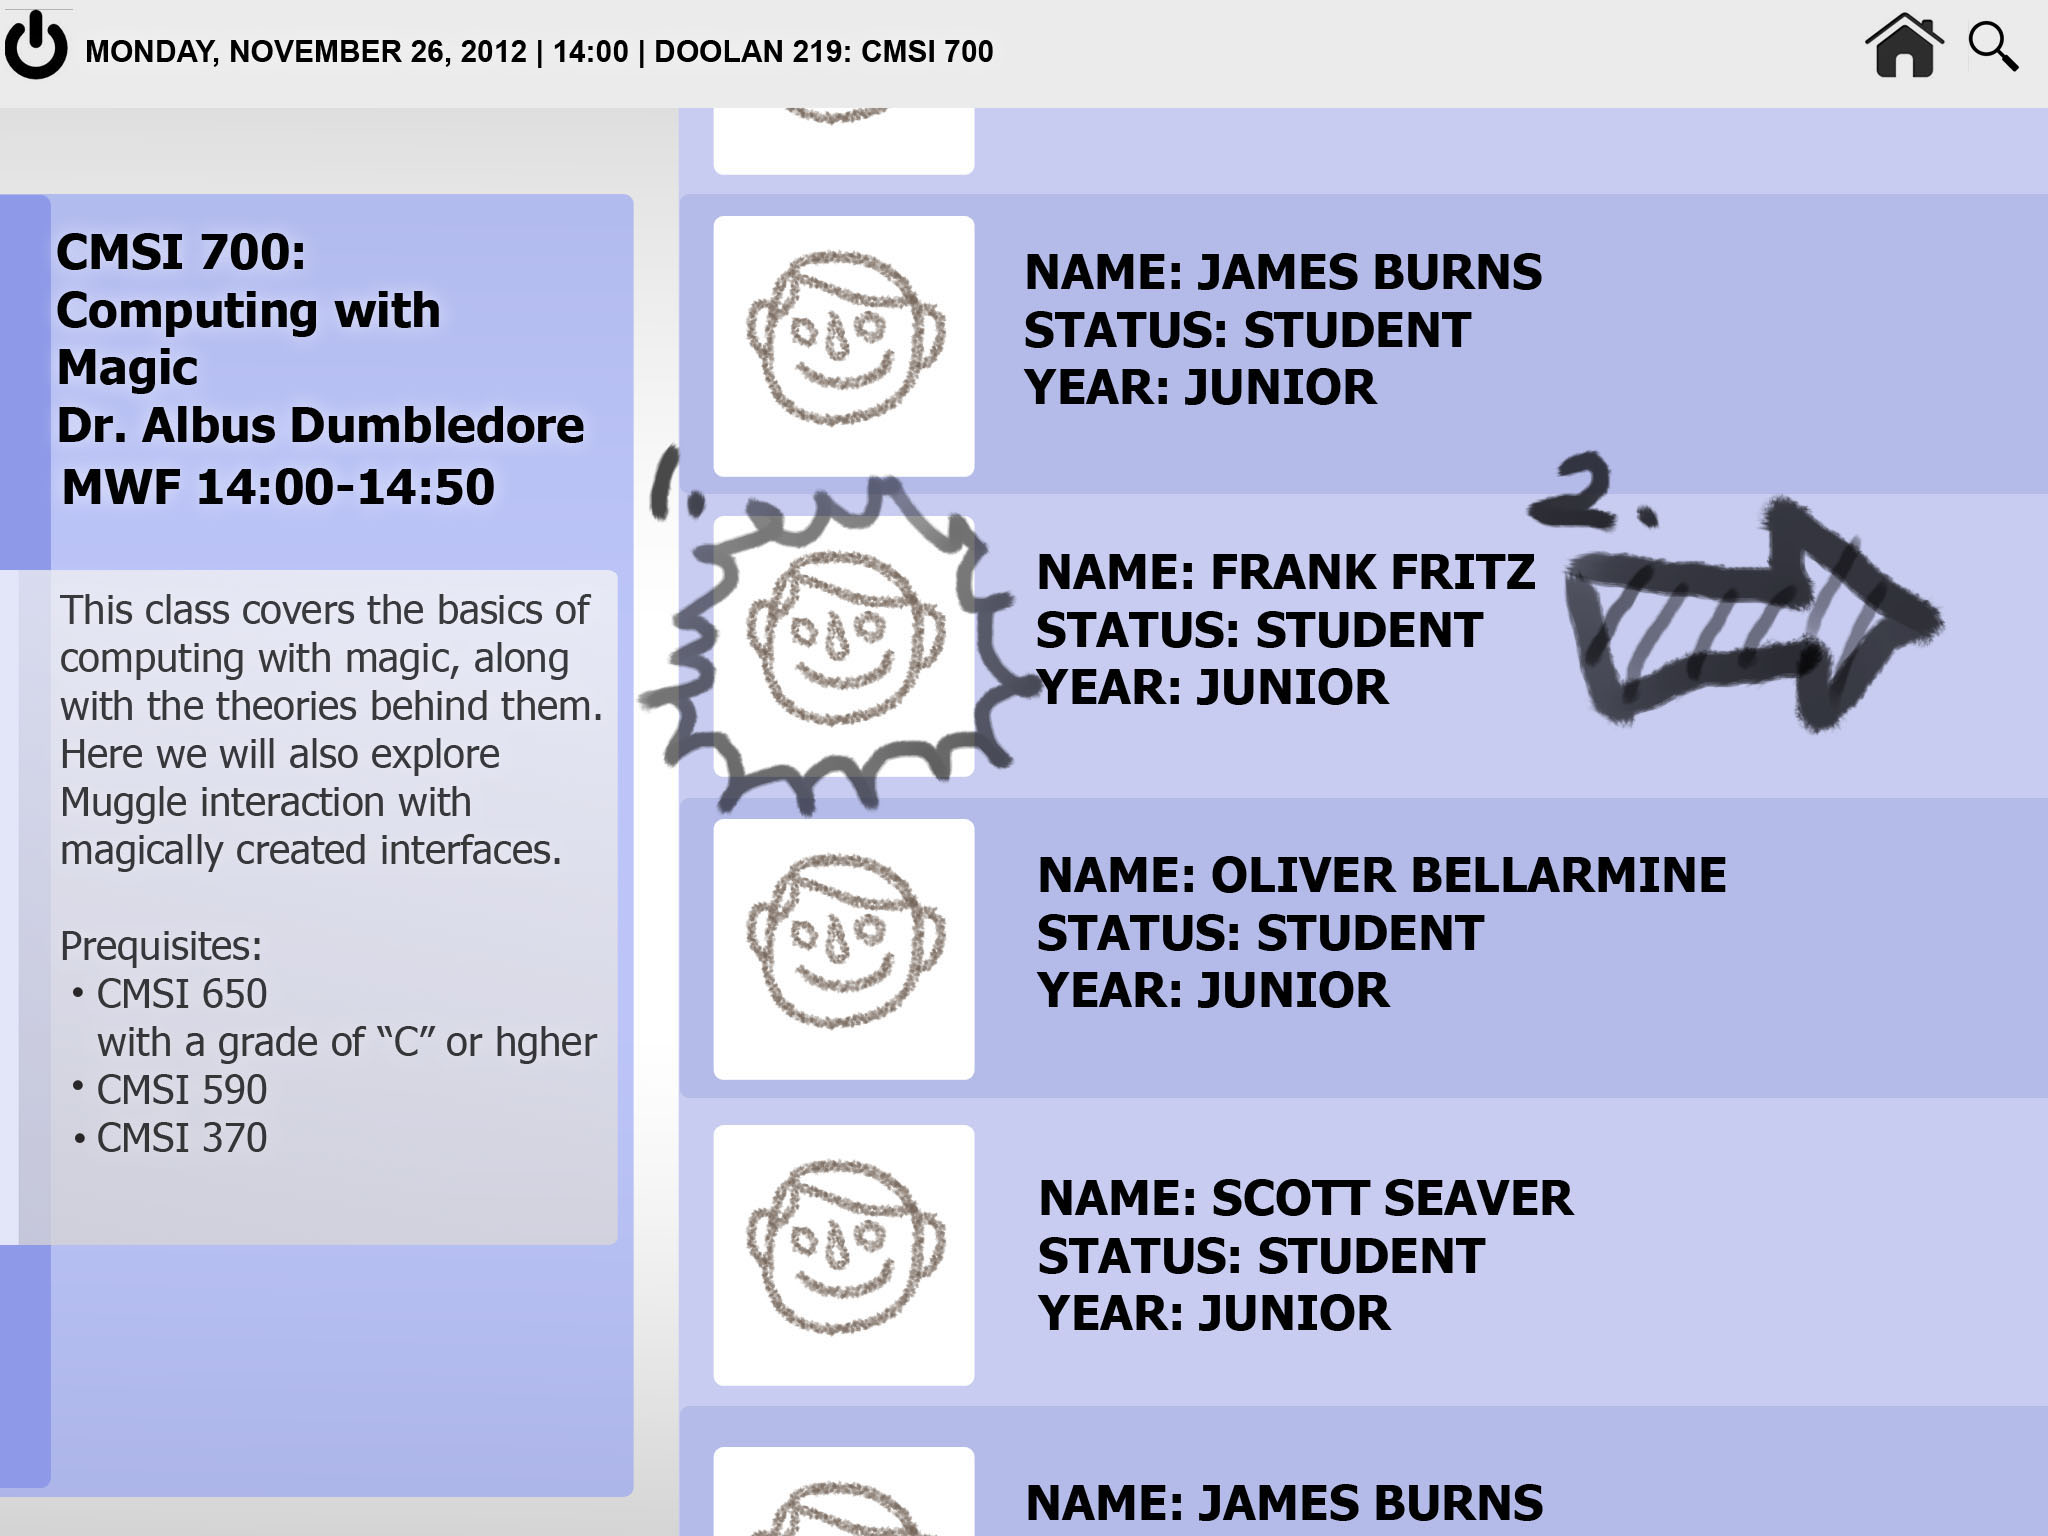
\includegraphics[width=\textwidth]{DESK}
\end{figure}
 

\section*{Learnability}
In addition to the simplicity of the design, the first time a user logs on using a device, they will experience a walkthrough.  This is in order to make sure that the user has no confusion with the system, thus improving user ability and eliminating errors, which is one of the most important principles of interface design. \cite{dondi12}   A pop-up will show with all newly visited screens, explaining key points, and how to maneuver through each page.  This feature turns off after the user has completed the tutorial (closed each pop-up and completed each action detailed by the pop-up), but can be turned on again in a toggle switch in the pull-down menu.  

\begin{thebibliography}

\bibitem{dondi12}
    John Dionisio,
    CMSI370: Interaction Design,
    2012

\bibitem{terror09}
    Diego Terror,
    \emph{Lessons From Swiss Style Graphic Design}.
    Smashing Design,
    \url{http://www.smashingmagazine.com/2009/07/17/lessons-from-swiss-style-graphic-design/},
    July 17, 2009

\bibitem{w3c07}
    W3C, Anne Van Kersteren, Maciej Stachowiak,
    \emph{HTML Design Principles}.
    \url{http://www.w3.org/TR/html-design-principles/},
    November 27, 2007


\end{thebibliography}

\end{document}